% This file was created by matlab2tikz.
%
\definecolor{mycolor1}{rgb}{0.00000,0.44700,0.74100}%
%
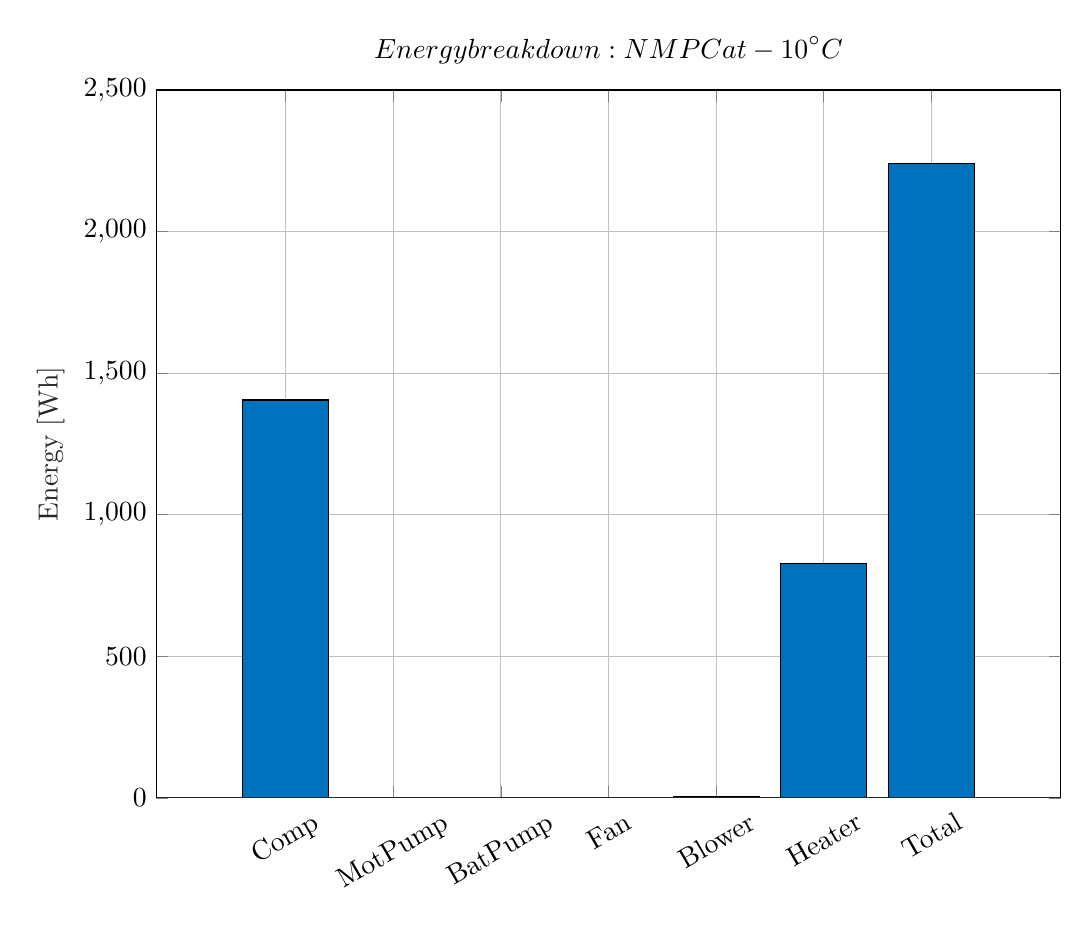
\begin{tikzpicture}

\begin{axis}[%
width=4.521in,
height=3.539in,
at={(0.758in,0.508in)},
scale only axis,
bar shift auto,
xmin=-0.2,
xmax=8.2,
xtick={1,2,3,4,5,6,7},
xticklabels={{Comp},{MotPump},{BatPump},{Fan},{Blower},{Heater},{Total}},
xticklabel style={rotate=30},
ymin=0,
ymax=2500,
ylabel style={font=\color{white!15!black}},
ylabel={Energy [Wh]},
axis background/.style={fill=white},
title style={font=\bfseries},
title={$\text{Energy breakdown: NMPC at -10}^\circ\text{C}$},
xmajorgrids,
ymajorgrids
]
\addplot[ybar, bar width=0.8, fill=mycolor1, draw=black, area legend] table[row sep=crcr] {%
1	1405.2176001022\\
2	2.68767321713351\\
3	2.13953161509665\\
4	0.963089139207336\\
5	3.67859287350085\\
6	826.868717115656\\
7	2241.55520406279\\
};
\addplot[forget plot, color=white!15!black] table[row sep=crcr] {%
-0.2	0\\
8.2	0\\
};
\end{axis}
\end{tikzpicture}%